\documentclass{CUP-JNL-DTM}%

%%%% Packages
\usepackage{graphicx}
\usepackage{multicol,multirow}
\usepackage{amsmath,amssymb,amsfonts}
\usepackage{mathrsfs}
\usepackage{amsthm}
\usepackage{rotating}
\usepackage{appendix}
\usepackage[numbers]{natbib}
\usepackage{ifpdf}
\usepackage[T1]{fontenc}
\usepackage{newtxtext}
\usepackage{newtxmath}
\usepackage{textcomp}
\usepackage{xcolor}
\usepackage{lipsum}
\usepackage[colorlinks,allcolors=blue]{hyperref}

\newtheorem{theorem}{Theorem}[section]
\newtheorem{lemma}[theorem]{Lemma}
\theoremstyle{definition}
\newtheorem{remark}[theorem]{Remark}
\newtheorem{example}[theorem]{Example}
\numberwithin{equation}{section}

\newcommand{\Julia}{\texttt{Julia} }

% \usepackage{lineno}
% \linenumbers

%\jname{Physics/Math}
\articletype{CAPSTONE PROJECT}
%\artid{20}
%\jyear{2022}
%\jvol{}
%\jissue{}
%\raggedbottom


\begin{document}

\begin{Frontmatter}

\title[Article Title]{Using Scientific Machine Learning to solve Partial Differential Equations}

\author[1]{Miles Cochran-Branson}\orcid{0000-0002-8514-4315}
% \author[2]{Author Name2}\orcid{0000-0001-8823-831X}
% \author[2]{Author Name3}\orcid{0000-0002-0251-345}

\authormark{Cochran-Branson, M. \textit{et. al}}

\address[1]{\orgdiv{Department of Physics and Mathematics}, \orgname{Lawrence University}, \orgaddress{\city{Appleton}, \state{WI}}}%, \postcode{54911}, \country{USA}}}

%\address[2]{\orgdiv{Division}, \orgname{Organization}, \orgaddress{\city{City}, \postcode{Pincode}, \state{State},  \country{Country}}. \email{name2@email.com}}

\keywords{SciML, Scientific Computing, ML/AI, PINN, PDEs}

\abstract{Here is my abstract!}

\end{Frontmatter}

\localtableofcontents

%% ---------------------------------------------------------------
%% Text Body!!

\section{Introduction}

Machine learning and scientific computing are two prominent fields with applications in physics, mathematics, and computer science. In the past several years, potential has been seen in combining the fields of machine learning and scientific computing to overcome two potential problems: lack of data, and solving diffenetial equations. \cite{karniadakisPhysicsinformedMachineLearning2021}

\section{Machine Learning}


\subsection{Neural Networks}

A neural network is simply a function. 

\begin{figure}
\centering
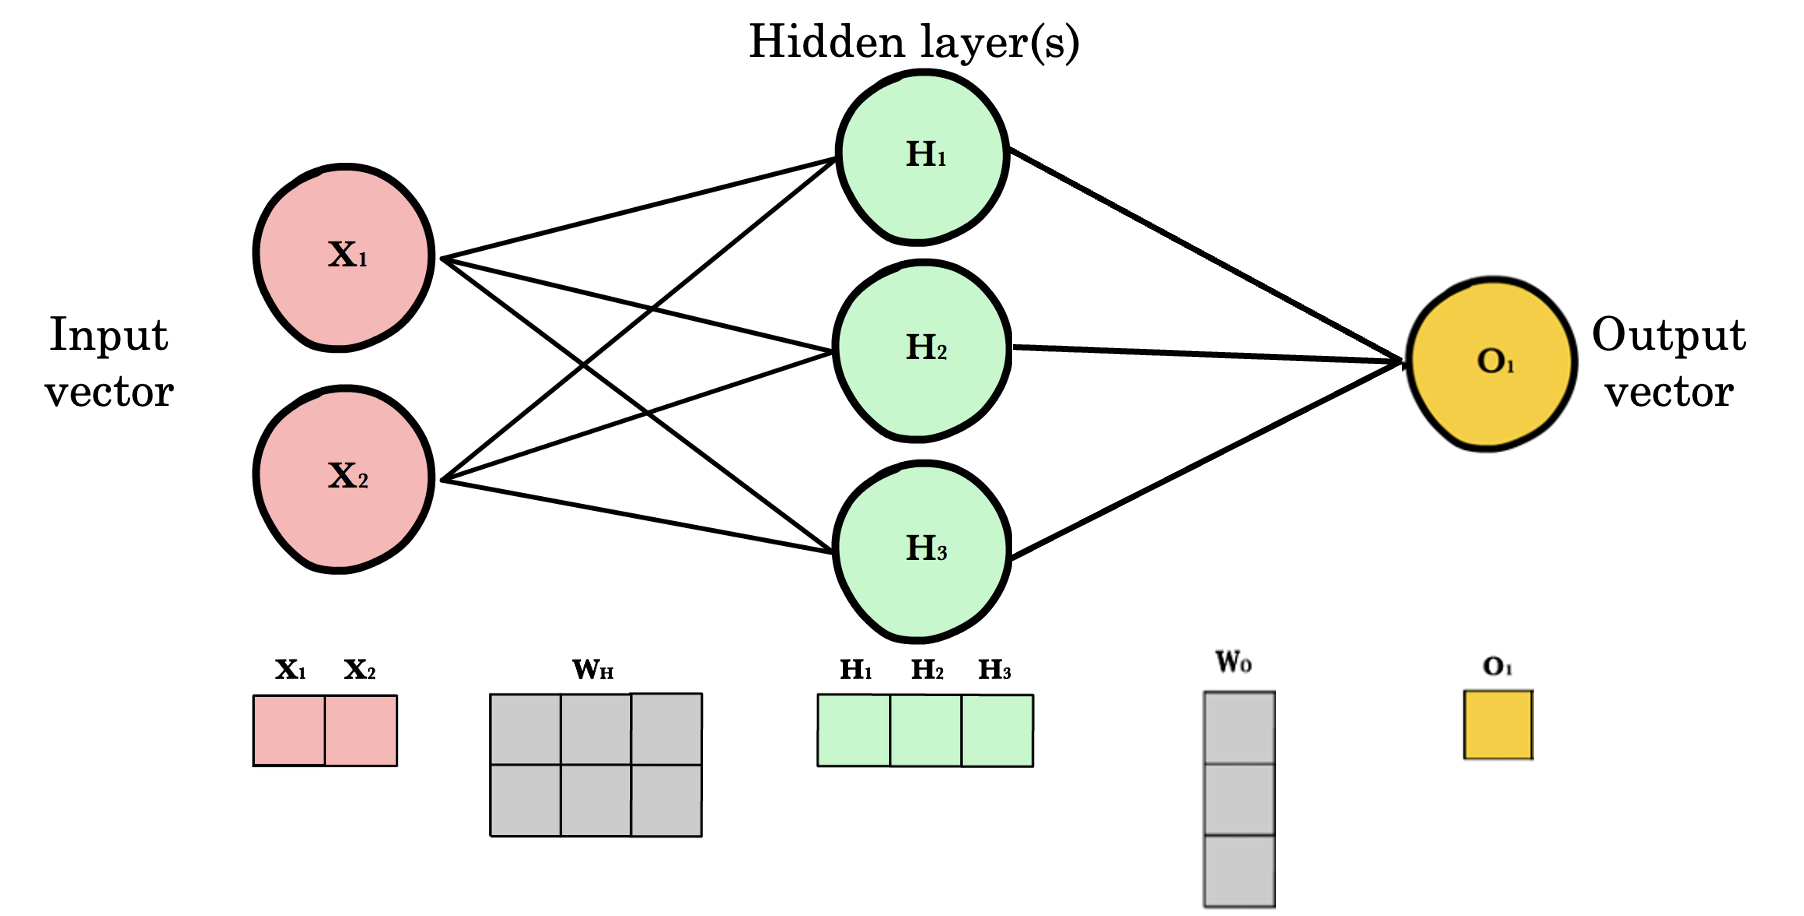
\includegraphics[width=0.7\linewidth]{figures/NN_example.png}
\caption{An example of a simple neural network with two inputs, one hidden layer with three nodes, and a single output. The network is defined by the weights connecting the layers which are represented as matrices. At each node, the weights are passed to a function called the \emph{activation function} which scales the weights appropriately. In principle, the size of the network can change in every dimension. }
\label{fig:NNexample}
\end{figure}

\subsection{Training Neural Networks}

\subsection{The Universal Approximation Theorem}

Thang that makes everything work!

\begin{theorem}

Consider $x \in \Omega$ and let $u(x)$ be a regular function and $N(x,w)$ be a neural network with weights $w$. Then we can find some arbitrarily small $\epsilon \in \Omega$ such that 

\begin{equation}
	||N(x,w) - u(x)|| < \epsilon. 
\end{equation}

\end{theorem}

\section{Solving ODEs with Physics-Informed Neural Networks}

\section{Solving PDEs with Physics-Informed Neural Networks}

We now turn out attention to solving partial different equations using techniques from scientific machine learning. We will use the package \texttt{NeuralPDE.jl} \cite{zubovNeuralPDEAutomatingPhysicsInformed2021} to solve some examples. 

Consider a partial differential equation given by 

\begin{equation}
	f(u(x); \lambda) = 0
\end{equation}
where $x \in \Omega$ are the independent variables in the space $\Omega$, $u(x)$ is the solution, $f$ is some non-linear function acting on $u$ and $\lambda$ are the parameters of the equation. To solve with a neural network $N(x, w)$ where $N$ is a neural network with weights $w$, we want to fulfill 

\begin{equation}
	f(N(x, w); \lambda) \approx 0.
	\label{eqn:NNapprox}
\end{equation}
The universal approximation theorem tells us that this should be possible. The error of the above equation is then given by 

\begin{equation}
	L(w) = \int_{\Omega} ||f(N(x,w); \lambda)||\,dx. 
	\label{eqn:NNloss}
\end{equation}
We have suggestively named the error $L$ as we can use this function as a loss function in training our neural network $N$ by attempting to minimize $L$. Our computational problem then reduces to the problem of evaluating the integral in Eqn. \ref{eqn:NNloss}. Notice that in practical problems, we apply boundary conditions $b_i$ on $\partial \Omega \in \Omega$. In order to use these in our neural network, we add in these conditions to our loss function giving us 

\begin{equation}
	L(w) = \sum_i\int_{\Omega\setminus\partial\Omega} ||f_i(N(x,w); \lambda)||\,dx + \sum_i\int_{\partial\Omega} ||b_i(N(x,w); \lambda)||\,dx.
	\label{eqn:complete_loss} 
\end{equation}
where we have generalized the problem to a system of coupled differential equations $f_i$. 

There are several different methods for evaluating the above integral namely: grid approximation techniques, stochastic grid approximation techniques, and machine learning (quadrature) techniques. A simple grid approximation takes the space $\Omega$ and divides it into units of volume $\Delta V$ with a specific length. The PDE is evaluated at each of this points and scaled by the volume, thus our integral is computed via 

\begin{equation}
	\int_{\Omega} ||f(N(x,w); \lambda)||\,dx = \sum_i \Delta V ||f(x_i)||.
\end{equation}
This method has two main disadvantages: 1) as the dimension of the problem increases, the number of points we sample increases exponentially in order to maintain the same granularity and 2) no evaluation of the integral is done between grid points, thus information can be quickly lost. To solve the second problem, we can use stochastic methods of sampling---i.e., use Monte Carlo techniques to evaluate the integral. This can be described by 

\begin{equation}
	\int_{\Omega} ||f(N(x,w); \lambda)||\,dx = \alpha \sum_i ||f(x_i)||.
\end{equation}
for some scaler $\alpha$. As we simply want to minimize this integral, there is no need to specify $\alpha$. This problem still suffers from dimensionality exponentially increasing. Thus, we turn to a third method: quadrature training with a neural network. Several processes for specifying quadrature are described in \cite{riveraQuadratureRulesSolving2022}. These are typically of the form 

\begin{equation}
	\int_{\Omega} ||f(N(x,w); \lambda)||\,dx = \sum_i \alpha_i ||f(x_i)||\,dx.
\end{equation}
In the implementation via \texttt{NeuralPDE.jl}, a neural network is solved via \texttt{Integrals.jl} which calls the \Julia differential equation solver \cite{rackauckasDifferentialEquationsJlPerformant2017} to find the correct sampling points $x_i$ and weights $\alpha_i$ in an implementation of Gaussian quadrature rules. 

\begin{example}

Consider the system of PDEs given by 

\begin{equation}
    \begin{split}
        \partial_t u_1 & = \partial_x^2 u_1 - u_2 \partial_x u_1 + u_1^2 - 2\int_0^1 u_1^2 \,dx \\
        0 & = \partial_x u_2 - u_1
    \end{split}
\end{equation}
for $0 < x < 1$ and $t > 0$. We emply the following initial condition

\begin{equation}
    u_1(0,x) = \cos \pi x
\end{equation}
and the following boundry conditions

\begin{equation}
    \partial_x u_1(t,0) = \partial_x u_1(t,1) = u_2(t,0) = u_2(t,1) = 0. 
\end{equation}
This system is solved in the paper \cite{benhammoudaAnalyticalSolutionsSystems2014} with the solution

\begin{equation}
    \begin{split}
        u_1(t,x) & = e^{-\pi^2t}\cos \pi x \\
        u_2(t,x) & = \frac{1}{\pi}e^{-\pi^2t} \sin \pi x. 
    \end{split}
\end{equation}

\end{example}

\begin{example}

Consider the PDAE given by 

\begin{equation}
    \begin{split}
        \partial_t^2 u_1 & = \partial_x^2 u_1 + u_3 \sin \pi x \\
        \partial_t^2 & = \partial_x^2 + u_3 \cos \pi x \\
        0 & = u_1 \sin \pi x + u_2 \cos \pi x - e^{-t}
    \end{split}
\end{equation}
on the intervals $0 < x < 1$, $t > 0$. We employ the following initial conditions

\begin{equation}
    \begin{split}
        u_1(0,x) & = \sin \pi x \\
        \partial_t u_1(0,x) & = -\sin \pi x \\
        u_2(0,x)
    \end{split}
\end{equation}

\end{example}

\section{Conclusion}

%% ---------------------------------------------------------------
%% Extra stuffs!

\begin{Backmatter}

\paragraph{Acknowledgments}

Grateful for support of Pickett and Heaton + physics and mathematics EDU at LU! Huzzah!!

\paragraph{Data Availability Statement}
I'll upload all of my code to GitHub and put a link to that here!

\bibliography{references}
\bibliographystyle{ieeetr}

\end{Backmatter}

\end{document}
